%version of 07-18-19

\chapter{The Art of Counting:
Combinatorics, Probability, and Statistics}
\label{ch:prob-stat}
\label{ch:combinatorics}

We have named this chapter in honor of the great German mathematician
Gottfried Leibniz, \index{Leibniz (Leibnitz), Gottfried Wilhelm} whose
1666 doctoral thesis, ``{\it Dissertatio de Arte Combinatoria}''
\cite{Leibnitz}, gave us the now-common phrase, ``the art of
counting.''\footnote{While Leibniz is best known (at least among students of mathematics) for his
never-to-be-settled dispute with Isaac Newton \index{Newton, Isaac}
over prior discovery of the calculus, Leibniz's life was in fact
dedicated to a broad range of topics in mathematics and philosophy.}
The word ``counting'' in this context must be understood
much more broadly than in the vernacular: In days past, the phrase
encompassed much of the field known nowadays as {\it
  combinatorics}. \index{combinatorics}

This chapter is devoted to introducing the basics of three closely related mathematical
subfields: combinatorics, probability, and statistics.

\medskip

\noindent {\it Combinatorics} (Section~\ref{sec:counting}).\index{combinatorics}\index{counting}
Our introduction to combinatorics can be viewed in many ways
as a return to Chapter~\ref{ch:sets-BA-logic}'s study of
sets, especially finite sets.  Indeed, the first topics we cover in
this chapter involve looking at a set $S$ ``from the inside'', to determine
how many elements (of a certain type) set $S$ contains.

\medskip

\noindent {\it Combinatorial probability} (Section~\ref{sec:combinatorial-prob}).
The tools we develop for determining the cardinalities of finite sets
give us access to the important (and fun!)~field known as {\em
  combinatorial probability} \index{combinatorial probability}
(Section~\ref{sec:prob-stat}).  In reality, probability theory is an {\em applied} spin-off
of combinatorics.  In its most elementary---and, some might say, frivolous---form, combinatorial probability uses counting to 
answer questions such as:  Why does the game of\index{poker}
($5$-card) poker value three-of-a-kind\index{poker!three-of-a-kind} more highly than two-pair?\index{poker!two-pair}
Why did the designers of roulette tables add two (green) extra slots to\index{roulette table}
the red and black slots of the wheel?  By the end of the section. you will have the wherewithal to answer
myriad questions of this ilk.

In a more serious vein, the elements of probability theory and statistics infuse every area of
computing.
\begin{itemize}
\item
The practicality of many algorithms that are experientially efficient often results from the {\em distributions} of 
the inputs they encounter in ``real" situations.
\item
Design methodologies for complex electronic circuits must be aware of the {\em
  mean times to failure} of the critical components of the circuits.
\item
Sophisticated searching algorithms---and heuristic search strategies---must take into account the relative
{\em likelihoods} of finding one's goal by following the various search directions that one has access to.
\item
Analyzing and understanding large corpora of data require methodologies that build on the 
concepts of {\em clustering} and/or {\em decomposition}.
\end{itemize}
Every student whose life will be touched by computing---which nowadays means just about
every student---needs at least an introduction to the foundations of
probability to even understand, all the more so to master, the terms highlighted in the preceding bulleted items.

\medskip

\noindent {\it Statistics} (Section~\ref{sec:statistics}).\index{statisticas}
Just as engineering can be viewed as the ``applied'' sibling of science, {\it statistics} can be viewed as 
the ``applied'' sibling of probability.  Whereas combinatorial probability will give the reader the ability to
calculate the likelihoods of various events' happening, statistics looks as the events ``in the large", by focusing on
parameters---aptly called ``statistics"---that measure quantities such as\index{statistical moments}
\begin{itemize}
\item
{\em means, medians}, and {\em modes}: different ways to embody concepts 
such as {\em averages) and {\em likelihood}.  These are attempts to find a single value that captures the essence
of many observed instances; they are often called the {\it first statistical moments}.
\index{statistical moments!means}\index{statistical moments!first moments}}
\item
{\em variances} and {\em standard deviations}: two closely related ways of measuring the error incurred by
employing first statistical moments such as means; they are often called the {\it second statistical moments}.
\index{statistical moments!variance}\index{statistical moments!standard deviation}
\item
{\em higher moments}: successive ways of measuring the errors incurred by
employing lower statistical moments to describe observed measurements.
\end{itemize}




\section{The Elements of Combinatorics}
\label{sec:counting}

This section contains two quite distinct, but closely related, lessons about counting.  The first lesson
is in the form of a single important example.  In Section~\ref{sec:b-ary strings}, we exploit the special
structure of {\em strings} to count the number of length-$n$ strings over fixed-size alphabets; and we 
extend this ability to other objects whose structures can be {\em encoded} as strings---notable the power-sets
of finite sets.  Then, in Section~\ref{sec:count-by-structure}, we illustrate how to count within sets that
are ``complex" in the sense of being formed from other sets by using the algebraic operations on sets that
we discuss in Section~\ref{sec:operations-on-sets}.


\subsection{Counting Binary Strings and Power Sets}
\label{sec:b-ary strings}
\index{strings!$b$-ary strings}
\index{strings!counting $b$-ary strings}

\begin{prop}
\label{thm:b-ary strings}
For every integer $b > 1$, there are $b^n$ $b$-ary strings of length
$n$.
\end{prop}

\begin{proof}
The asserted numeration follows most simply by noting that there are
always $b$ times as many $b$-ary strings of length $n$ as there are of
length $n-1$.  This is because we can form the set of $b$-ary strings
of length $n$ as follows.  Take the set $A_{n-1}$ of $b$-ary strings
of length $n-1$, and make $b$ copies of it, call them $A^{(0)}_{n-1},
A^{(1)}_{n-1}, \ldots, A^{(b-1)}_{n-1}$.  Now, append $0$ to every
string in $A^{(0)}_{n-1}$, append $1$ to every string in
$A^{(1)}_{n-1}$, \ldots, append $\bar{b} = b-1$ to every string in
$A^{(b-1)}_{n-1}$.  The thus-amended sets $A^{(i)}_{n-1}$ are mutually
disjoint (because of the terminal letters of their respective
strings), and they collectively contain all $b$-ary strings of length
$n$.  \qed
\end{proof}

\medskip

Proposition~\ref{thm:b-ary strings} has a corollary whose proof is much more important than its
statement.   By employing the {\em characteristic vectors} of sets, we invoke the case $b=2$ of 
Proposition~\ref{thm:b-ary strings} to determine how many subsets a finite set $S$ has---i.e., to
count the elements of $S$'s {\em power set}.  (All technical terms
come from Chapter~\ref{ch:sets-BA-logic}.)


\begin{prop}
\label{thm:power-sets}
The power set $\p(S)$ of a finite set $S$ contain $2^{|S|}$ elements.
\end{prop}

\begin{proof}
We begin by taking an arbitrary finite set $S$---say of $n$
elements---and laying its elements out in a line.  We thereby
establish a one-to-one correspondence between $S$'s elements and the positive
integers: there is the first element, which we associate with the
integer $1$, the second element, which we associate with the integer
$2$, and so on, until the last element along the line gets associated
with the integer $n$.

Next, we note that we can specify any subset $S'$ of $S$ by
specifying a length-$n$ {\em binary (i.e., base-$2$) string}, i.e., a
string of $0$'s and $1$'s.  The translation is as follows.  If an
element $s$ of $S$ appears in the subset $S'$, then we look at the
integer we have associated with $s$ (via our linear ordering of $S$),
and we set the corresponding bit-position of our binary string to $1$;
otherwise, we set this bit-position to $0$.  In this way, we get a
distinct subset of $S$ for each distinct binary string, and a distinct
binary string for each distinct subset of $S$.  (We thus have a {\em bijection}.)

Let us pause to illustrate our correspondence between sets and strings
by focussing on the set $S = \{a,b,c\}$.  Just to make life more
interesting, let us lay $S$'s elements out in the order $b,a,c$, so
that $b$ has associated integer $1$, $a$ has associated integer $2$,
and $c$ has associated integer $3$.  We depict the elements of $\p(S)$
and the corresponding binary strings in the following table.
\begin{center}
\fbox{
\begin{tabular}{c|c|c}
Binary string & Set of integers & Subset of $S$ \\
\hline
$000$ & $\emptyset$ & $\emptyset$ \\
$001$ & $\{3\}$     & $\{c\}$ \\
$010$ & $\{2\}$     & $\{a\}$ \\
$011$ & $\{2,3\}$   & $\{a,c\}$ \\
$100$ & $\{1\}$     & $\{b\}$ \\
$101$ & $\{1,3\}$   & $\{b,c\}$ \\
$110$ & $\{1,2\}$   & $\{a,b\}$ \\
$111$ & $\{1,2,3\}$ & $\{a,b,c\} =S$
\end{tabular}
}
\end{center}

Back to the Proposition: We have verified the following: {\em The
  number of length-$n$ binary strings is the same as the number of
  elements in the power set of $S$!}  The desired numeration thus
follows by the ($b=2$) instance of Proposition~\ref{thm:b-ary
  strings}.  \qed
\end{proof}

\bigskip

\noindent \fbox{
\begin{minipage}{0.95\textwidth}
The binary string that we have constructed to represent each set of
integers $N \subseteq \{0, 1, \ldots, n-1\}$ is the {\it
(length-$n$) characteristic vector}\index{characteristic vector}
{\it of the set} $N$.  Of course, the finite set $N$ has
characteristic vectors of all finite lengths.  Generalizing this idea,
{\em every} set of integers $N \subseteq \N$, whether finite or
infinite, has an {\em infinite} characteristic vector, which is formed
in precisely the same way as are finite characteristic vectors, but
now using the set $\N$ as the base set.
\end{minipage}
}


\subsection{Counting Based on Set Algebra}
\label{sec:count-by-structure}
\index{counting sets!based on set algebra}

In this section, we assume that we know the cardinalities of certain {\em finite} sets---call
them $A$, $B$, and $C$---and we want to know the cardinality of a new set which is formed
from these sets by the basic operations of the algebra of sets, as discussed in
Section~\ref{sec:operations-on-sets}.  There are a few commonly invoked counting laws
which should be in your toolkit.

\begin{itemize}
\item
{\it The bijection rule}\index{The bijection rule for counting elements of sets}

\smallskip

If the elements of set $A$ can be put into bijective correspondence with the elements of set
$B$, then sets $A$ and $B$ have the same cardinality.  Symbolically, $|A| = |B|$.

\item
{\it The addition rule} \index{The addition rule for counting elements of sets}

The addition rule is also known as the {\it Law of inclusion and exclusion}.
\index{the law of inclusion and exclusion}\index{inclusion and exclusion law}

\smallskip

One can compute the cardinalities of unions of sets by adding and/or subtracting
the cardinalities of the individual sets.  For any sets $A$ and $B$.
\[ |A \cup B| \ \ = \ \ |A|  \ + \ |B| \ - \ |A \cap B| \]
Specifically:
  \begin{itemize}
  \item
If $A$ and $B$ are {\em disjoint}---i.e., $A \cap B = \emptyset$, so that
have no common elements---then $|A \cup B| = |A| + |B|$.

 \item
if $A$ and $B$ {\em intersect}---i.e., $A \cap B \neq \emptyset$, so that $A$ and
$B$ share some elements---then $|A \cup B|  =  |A|  + |B| - |A \cap B|$.

This formula {\em includes} the elements of both sets and the {\em excludes} the sets'
shared elements, which are double-counted by the inclusion.  (You can see the origin of the
name ``the law of inclusion and exclusion.")
 \end{itemize}
Figs.~\ref{fig:unionSetsInit} and~\ref{fig:unionSets} illustrate how to generalize the preceding equations to
collections of three sets; going beyond three adds complexity that is clerical but not conceptual.
\begin{figure}[htb]
\begin{center}
        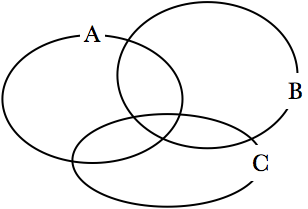
\includegraphics[scale=0.35]{FiguresMaths/3sets}
        \caption{Three sets, $A$, $B$ and $C$, in ``general" position, i.e., with all possible overlaps.}
        \label{fig:unionSetsInit}
\end{center}
\end{figure}
\begin{figure}[htb]
\begin{center}
        
\includegraphics[scale=0.35]{FiguresMaths/RuleAdditive}
        \hspace{1cm}
        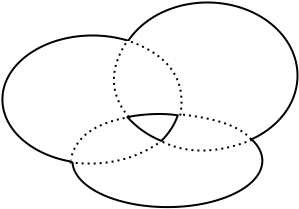
\includegraphics[scale=0.35]{FiguresMaths/RuleAdditive2}
        \caption{The union of sets $A$, $B$, and $C$ (left), and their intersections (right).}
        \label{fig:unionSets}
\end{center}
\end{figure}
In order to draw explicit expressions that express the content of  Fig.~\ref{fig:unionSets}, one must apply the Law of
{\em inclusion and exclusion} in multiple ways, as we compensate for the 
pairwise and triple intersections among  sets $A$, $B$, and $C$.  A careful reckoning using the figure 
indicates that
\[ |A \cup B \cup C| \ \ = \ \ 
\big(|A| + |B| + |C| \big) - \big( |A \cap B| + |A \cap C| + |B \cap C| \big) + |A \cap B \cap C|. \]
In particular, we begin by {\em including} the union; then we {\em exclude} the pairwise intersections, which
were double-counted; and we finally {\em include} the triple intersection, which was doubly excluded.

\item
{\em The multiplication rule} \index{The multiplication rule for counting elements of sets}

This rule tells us how to count the cardinalities of Cartesian products of sets, as
illustrated in Fig.~\ref{fig:cartesianproduct}.
\[ |A \times B| \ \ = \ \ |A| \cdot |B| \]
The multiplication rule extends immediately to multiplicities of sets; e.g., for three sets:
\[  |A \times B \times C| \ \ = \ \ |A| \cdot |B| \cdot |C| \]

As an important special case, we note that
\[ |A \times A \times \cdots  \times A| \ \mbox{ ($p-1$ times)}  \ \ = \ \ |A|^p \]
The exciting feature in this last equality is that the set
 \[ A \times A \times \cdots  \times A  \mbox{($p-1$ times)} \]
is a (nonstandard) way of representing the set of length-$p$ strings of elements of $A$.
Thereby, the multiplication rule gives us an alternative way to 
view---and to prove---Proposition~\ref{thm:b-ary strings}.
\end{itemize}

\bigskip

As we move forward, we shall encounter many other ways of counting the elements of sets,
most importantly by using operations involving {\it selection} and {\it rearrangement}.  As we
proceed with this new material, we will encounter old friends, often wearing new clothing.  We
will renew our acquaintance with the factorial operation and with binomial coefficients; we will
have cause to recall the pigeonhole principle in new settings.  And, we will discover new domains
of application, as we move beyond ``pure" mathematics to the applications of mathematical
laws in domains related to probability and statistics.
Let us begin our journey.

\subsection{Counting Based on Set Arrangement and Selection}
\label{sec:set-arrangement}

This section introduces the primary operations that are used for arranging finite sets as we
establish a base for studying combinatorial probability.  The importance of set-arrangement
in this context results from the common practice of defining
discrete probability/likelihood as a counting problem---most specifically, of defining the ratio:
\[ 
\frac{\mbox{number of ways of achieving a targeted event $E$}}{\mbox{number of possible events}}
\]
as the ``probability" of event $E$.

\medskip

We focus on three notions of arranging, and selecting from, a set of $n$ objects:
\[ \{ x_1, x_2, \ldots , x_n\} \]
When useful for explaining some idea, we sometimes identify the $x_i$ as some specific type
of objects, such as numbers, but generally we do not exploit any specific
characteristics of the $x_i$.

\medskip

\noindent {\it Permutations}.\index{permutation}
A permutation of an $n$-element set $A$ is a {\em fixed ordering} of the elements of $A$:  
each element of $A$ appears precisely once in the ordering.  We denote a permutation
of an $n$-element set via the notation
\[ (x_1,x_2, \ldots , x_n) \]
where each $x_i$ appears precisely once.  Note that we use parentheses for grouping,
as in ``$(3,2,1,4)$", instead of braces, as in ``$\{3,2,1,4\}$", to emphasize the ordering.  In
particular,
\[ \{3,2,1,4\} \ = \ \{1,2,3, 4\} \ \ \ \mbox{ but } \ \ \ (3,2,1,4) \ \neq \ (1, 2, 3,4) \]

\medskip

In terms of problems relating to {\em selecting}\index{selection problems}
$m$ elements from a set of $n \geq m$ elements, permutations give rise to the most demanding
genre of selection: {\em They demand accounting for both the {\em identities}
of the selected elements and the {\em orders} in which the elements were selected.}

\medskip

It is a straightforward exercise to count the number of permutations of $n$ items.

\begin{prop}
\label{thm:no-permutation}
The number of permutations, $P(n)$, of a $n$-element set equals $n!$
\end{prop}

\begin{proof}
Just for the practice, we describe two inductive proofs of this simple result, based on two
quite-distinct eays of constructing permutations.  We merely
sketch the inductions underlying the proofs, leaving details for your practice.

\medskip

\noindent {\bf 1.}
To construct a permutation of the $n$-element set $\{ x_1, x_2, \ldots , x_n\}$:
\begin{itemize}
\item
Select the first element of the permutation in $n$ ways: any $x_i$ will work.
\item
Having selected the first item, we are left with the $(n-1)$-element version of the problem.
\end{itemize}
We thereby find that $P(n)$ is specified recursively as follows.
\[
P(n) \ = \ \left\{
\begin{array}{cl}
1 & \mbox{ if } \ n=1 \\
n \cdot P(n-1) & \mbox{ if } \ n>1
\end{array}
\right.
\]
By elementary reasoning, we find that $P(n) \ = \ n!$.

\bigskip

\noindent {\bf 2.}
To construct a permutation of the $n$-element set $A = \{ x_1, x_2, \ldots , x_n\}$:
\begin{itemize}
\item
Assume, inductively, that you are given a fixed 
permutation $(x_1, \ldots , x_{n-1})$ of an $(n-1)$-element subset $A'  \subset A$,
chosen somehow from among the $(n-1)!$ possible orderings of set $A'$.  (Note
the thinly veiled use of induction.)
\item
Take element $x_n$, which does not belong to $A'$, and place it into the ordering of $A'$
that you are given.  You can place $x_n$ in any of $n$ positions in the new permutation:
  \begin{itemize}
  \item
before (i.e., to the left of) all of the preplaced elements of $A'$;
  \item
after (i.e., to the right of) all of the preplaced elements of $A'$;
  \item
in between any adjacent preplaced elements of $A'$.
  \end{itemize}
Each of the preceding $n$ choices creates a unique permutation of the $n$-element set $A$.
\end{itemize}
Using arithmetic virtually identical to case {\bf 1} verifies that $P(n) \ = \ n!$.

\medskip

\noindent
Other variants on the preceding proof themes will undoubtedly occur to you.   \qed
\end{proof}


%%%%%%%%%%%%%%%%%%%%%%%

\medskip

\noindent {\it Combinations}.\index{combination}
Within the context of selection problems, combinations are the ``next step down" in
strictness from permutations.  When one selects $m$ items from a set of $n \geq m$ items,
combinations are concerned with the {\em identities} of the elements selected, but not with 
the order in which they elements are chosen.

\noindent (This willingness to ignore order gives a big hint about how to count the number of
combinations of $m$ items chosen from $n$.  Can you figure out how to use the hint before
we get to Proposition~\ref{thm:no-combination}?)

\medskip

Factorials play as essential a role in combinational selection as in permutational selection, but
now it plays a {\em dual} role: choosing the identities of the selected elements {\em and} factoring out
the order in which the elements were selected.  The binomial coefficients that we introduced
in Section~\ref{sec:binomial-coeff} and that have arisen several times since then
throughout our journey are
(literally!) tailor made for this genre of selection problem.  Recall that
\[ {n \choose m} \ = \ \frac{n(n-1)\cdots(n-m)}{m!} \ = \  \frac{n!}{m!(n-m)!} 
\]

\begin{prop}
\label{thm:no-combination}
The number of ways of selecting $m$ elements from a set of $n \geq m$ elements, while 
ignoring the order in which the $m$ elements were selected is $\displaystyle {n \choose m}$.
\end{prop}

\begin{proof}
The number of {\em ordered} ways of selecting $m$ elements from a set of $n \geq m$
elements is 
\begin{equation}
\label{eq:combination}
n \cdot (n-1) \cdot \cdots \cdot (n-m+1) \ = \ \frac{n!}{(n-m)!}
\end{equation}
To wit: One can select the first element in any of $n$ ways.  Having selected this element,
there are $n-1$ ways to choose the second element---and $n-2$ ways to choose the third
element, $n-3$ ways to choose the fourth element, and so on.

This method of numeration accounts for both the identity of the $i$th chosen element 
{\em and} the fact that it was the $i$th element chosen.  In other words, if element $x_1$
is the first element chosen,
and element $x_2$ is the second one chosen, then the two orders of selection
\[ x_1, \ x_2, \ \mbox{(a fixed order for the remaining $m-2$ selections)} \]
and 
\[ x_2, \ x_1, \ \mbox{(a fixed order for the remaining $m-2$ selections)} \]
are counted as separate events.  Easily, this overcounting uniformly expands each of the
events that we {\em do} want to account for by the factor $m!$, for this is the number of orders 
in which we could have selected the finally chosen $m$ elements.
 
This reasoning indicates that we can compensate for our overcounting by dividing the 
{\em ordered} tally (\ref{eq:combination}) by $m!$.  This compensation replaces tally
(\ref{eq:combination}) by $\displaystyle {n \choose m}$, whence the result.  \qed
\end{proof}

\bigskip

\noindent {\it Derangements}\index{derangement}

**HERE

In the cartesian product  $A \times A ... \times A$, there are words with multiple $a_i$.
For instance, considering $A=\{ 1,2,3 \}$, the element $(3,2,3,1)$ of $A^4$ contains twice the element $a_3=3$ 
or $(1,2,1,1)$ contains three times $a_1=1$. 
A natural question is to study what happens if we want only the words with different components?


Derangements of a set $A$ is a bijection without \textit{fixed points}.
This means that we donot allow an element to be associated to itself
or (using a more formal vocabulary), there is no cycle of length 1 in the strings of $A^n$
($n$ is the cardinal of $A$).

Let denote by $d(n)$ the number of derangements.
\medskip

Consider for instance the set $A = \{1,2,3 \}$, there are two derangements, namely
($1 \rightarrow 2$, $2 \rightarrow 3$, $3 \rightarrow 1$)
and 
($1 \rightarrow 3$, $2 \rightarrow 1$, $3 \rightarrow 2$).
\medskip

$d(1) = 0$ and $d(2) = 1$

$d(n) = (n-1) (d(n-1) + d(n-2))$

$d(n) = (-1)^n + n d(n-1)$
\bigskip

By the principle inclusion/exclusion, we show that the complexity is roughly of order $n!$

As the number of objects increases, the probability that none appears in its correct position approaches
$p=lim_{n \rightarrow \infty}\frac{d(n)}{n!}=\frac{1}{e}$. 

{\Denis Interesting: to be detailed in more details...}









\section{The Elements of Combinatorial Probability}
\label{sec:combinatorial-prob}


Perhaps the easiest and most engaging way to introduce ``probability
via counting" is by calculating the comparative likelihoods of various
deals in $5$-card poker and of various rolls of a pair of dice.  The
arithmetic required for this discussion is elementary and the
``application" to gambling of interest even to non-gamblers: ``Why is
such a deal in poker (say, a straight) worth more than another (say,
three of a kind)?"  One can also introduce in this setting concepts
such as randomness, bias, etc., that are so important in the design of
experiments and the analysis of their outcomes.


\subsection{Introduction to Probability}
\label{sec:prob-stat}


Elements of probability theory and statistics infuse every area of
computing.  The practicality of many algorithms that are
experientially the most efficient for their target tasks depend on the
{\em distribution} of inputs in ``real" situations.  Design
methodologies for crucial complex circuits must acknowledge the {\em
  mean times to failure} of the critical components of the circuits.
Sophisticated searching algorithms must take into account the relative
{\em likelihoods} of finding one's goal in the various optional search
directions.  Analyzing and understanding large corpora of data
requires a variety of methodologies that build on the concepts of {\em
  clustering} and/or {\em decomposition}.

A student needs at least an introduction to the foundations of
probability and statistics to even understand, all the more so to
master, the terms highlighted in the preceding paragraph.  We outline
many of the key concepts that a student must be exposed to in the
following subsections.

{\Denis Here we may be more precise about the content: the probabilities are built upon combinatoric rules, another interesting point is to distinguish between probability and statistics...}



\subsection{The Elements of Combinatorial Probability}

Perhaps the easiest and most engaging way to introduce ``probability
via counting" is by calculating the comparative likelihoods of various
deals in $5$-card poker and of various rolls of a pair of dice.  The
arithmetic required for this discussion is elementary and the
``application" to gambling of interest even to non-gamblers: ``Why is
such a deal in poker (say, a straight) worth more than another (say,
three-of-a-kind)?"  One can also introduce in this setting concepts
such as randomness, bias, etc., that are so important in the design of
experiments and the analysis of their outcomes.

Let recall that games can be characterized by pure gambling -- random games (dices and wheels), 
mental games (board games like chess or GO)
 {\Denis I don't know the english term for the games that challenge the mind...} 
and mixed ones (Backgammon, Bridge or Poker).
\medskip

Introducing discrete probability/likelihood as a ratio:
\[ 
\frac{\mbox{number of targeted events}}{\mbox{number of possible events}}
\]

We have several immediate consequences:

First, since the number of targeted events is lower than the number of all possible events,
the probability is lower than $1$. 

It is also positive, and a probability $0$ corresponds to the probability of an empty event.

An event is as probable as its probability is close to 1.

Using the additive rule, the probability of two distinct series of events is equal to the sum of the probabilities
of both events. 
In particular, the probability of two complementary events is equal to 1 (obtained by $p + (1-p)$).


\subsection{Illustration: Playing Poker}

Let us consider a usual deck of 52 cards composed of $n=13$ figures:

\textit{(2,3,4,5,6,7,8,9,10,Jack,Queen,King,Ace)} 

on the 4 colors \textit{(club, diamond, heart and spades)}.

The total number of possible \textit{hands} (i.e. set of the 5 cards owns by each player) is 
${32 \choose 5} = \frac{52!}{5! 47!} = 2 598 960$, this is a huge number of possibilities that makes the Poker game an interesting one.

The patterns that characterize the game in a hand can be classified by their number of occurrences.
Let survey briefly the principal ones.

\begin{itemize}
\item
There are only 4 different ways to form a royal flush (i.e. the 5 cards  \textit{(10,J,Q,K,Ace)} of the same color). 
Thus, the probability of getting such an hand is equal to $\frac{4}{2 598 960}$ that is one over $649740$, which is equal to $0.000154$.
\item
Now, let us calculate the number of hands within a straight flush, excluding the royal flush.

The reasoning is similar as for the royal flush, taking into account that there are $9$ possible series of $5$ consecutive cards
(from \textit{(Ace,2,3,4,5)}, \textit{(2,3,4,5,6)}, and so on --- shifted progressively --- to \textit{(9,10,J,Q,K)}).

Thus, as the flush requires to have the same color, there are $9 \times 4 = 36$ such hands. 
\item
Four-of-a-kind.

There are $13$ possible cards. There is a remaining card left that is any one among the 48 remaining ones.
Indeed, according to the multiplicative principle, it remains ${12 \choose 1}$ in each of the $4$ colors. 
Thus, $13 \times 48 = 624$, which corresponds to the probability $0.00256$.
\item
Three-of-a-kind and Full Houses.

The analysis of the first of these two patterns follows the same logic as for the Four-of-a-kind.
Again, there are as many possibilities of the $3$ base cards of the pattern than the number of cards in a color ($13$)
with only $3$ colors among the 4: ${4 \choose 3}$.
The two remaining cards should be different from the kind (and different from each other), 
thus, their number is to select $2$ among the $12$ remaining ones,
each one can take any colors (their number is $4^2$).
The final expression is:

$13.{4 \choose 3}.{12 \choose 2}.4^2 = 858$

For getting a Full House, the enumeration is close to the previous one, but there is a slight difference 
on the two remaining cards,
which here should by a pair (two of the same kind, that is only $1$ card among the $12$, 
this card can take any of the four colors),
thus:
\[ 13 \times {4 \choose 3} \times {12 \choose 1} \times 4 = 156 \]
\end{itemize}


\subsection{The Monty Hall Puzzle}
\label{sec:monty-hall}

The following real-life situation illustrates that reasoning
probabilistically is not easy and can be quite unintuitive.

We recall a popular tv show from the 1970s and 1980s, \textit{Let's
  Make a Deal}.\index{Let's Make a Deal} In one segment of the show, a
contestant was confronted by three doors, door (1), door (2), and door
(3); see Fig.~\ref{fig:MonthyHal-1}.
\begin{figure}[htb]
\begin{center}
        \includegraphics[scale=0.4]{FiguresMaths/MonthyHallInitial}
%            \includegraphics[scale=0.5]{FiguresProba/MonthyHallInitial}
        \caption{The three doors of \textit{Let's Make a Deal}.}
        \label{fig:MonthyHal-1}
\end{center}
\end{figure}
The contestant was told that a jackpot was behind one of the doors;
the other two hid less-desirable prizes.  The show's host, Monty Hall,
\index{Hall, Monty} invited the contestant to choose one of the doors:
she would receive whatever prize was behind the door she selected.

Since the door names are irrelevant to the story, let us assume that
the contestant chose door (1).  Before that selection was considered
final, Monty Hall would open {\em one of} doors (2) or (3), i.e., one
of the two {\em unchosen} doors.  Again for illustration, let us
assume that Monty opened door (3).  Assuming that the jackpot did {\em
  not} appear behind door (3), Monty now gave the contestant the
option of changing her initial choice, from door (1) to door (2).

What should the contestant do?  

Let us begin with intuition.  As the story began, the contestant had a
one-in-three chance of choosing the door that hid the jackpot.  As the
story progresses, is it conceivable that these odds change after door
(3) is shown not to hide the jackpot?  How could this be?

Well, the popular (well-named) columnist Marilyn von Savant
\index{von Savant, Marilyn} published an analysis that shows that
{\em it is better to change one's choice!}  Here is her reasoning,
enhanced by the illustration in Fig.~\ref{fig:MonthyHall-2}.
\begin{figure}[htb]
\begin{center}
        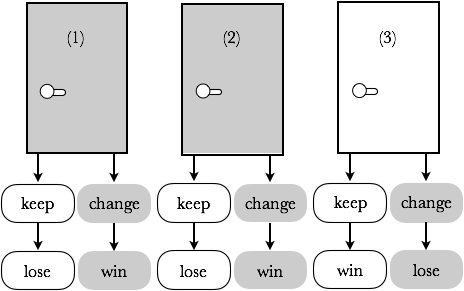
\includegraphics[scale=0.4]{FiguresMaths/MonthyHall}
%                \includegraphics[scale=0.4]{FiguresProba/Monthy}
        \caption{Suppose the jackpot is behind door (3). 
        If we select it, we lose if we change the initial choice.
        However, it is better to change if we select one of both other doors (1) or (2).}
        \label{fig:MonthyHall-2}
\end{center}
\end{figure}
We distinguish the two possible cases.
\begin{itemize}
\item
If the contestant had selected the jackpot-door at the beginning, then
holding on to this choice leads to the same probability of success as
she had from the beginning, namely, {\em one-third}.
\item
If the contestant had selected a wrong door at the beginning---which
occurs with probability {\em two-thirds}---then she will win the
jackpot if she now changes her initial (erroneous) choice.
%because now the choice in among two cases. 
\end{itemize}
Thus, quite unintuitively, the contestant should change her original
choice, based on the information she has now.

\smallskip

You can have fun by confronting your friends with this unintuitive
analysis.

\medskip

Of course, this is not just a trick!  It is a demonstration that you
can improve your chances of winning by taking advantage of all
available information!  The ``science'' behind this analysis is built
upon the topic of {\em conditional probability},
\index{conditional probability} in general and Bayes's Theorem in
particular. \index{Bayes's Theorem}  Both topics are beyond the scope
of this text: See \cite{Lee12} for a general presentation of this
topic and \cite{Bayes} for the original work.


\subsection{The Birthday Puzzle}
\label{sec:birthday-puzzle}
\index{birthday puzzle}

This section presents another application of the rules of enumeration
to the calculation of probabilities~\cite{DumasTrystram}.  The main
message with this application is: {\em it is sometimes easier to
  calculate the probability that an event {\em does not} occur than
  the probability that it {\em does} occur.}

\medskip

A common way for a teacher of a new class to establish rapport with
students is to determine whether any students share a birthday.  When
the class has (at least) around 30 students, the answer is usually
\textit{yes}.  The frequency of this response suggests that the
presence of birthday sharers is not mere chance!  If this is a
mathematics class, then there is a teaching opportunity here!  The
teacher and students can jointly derive an answer to the following
question.

{\it How many people must gather before the probability that some two share}

{\it a birthday reaches 50\%?}

\smallskip

\noindent
We now develop an answer to this question, based on the assumption
that all dates are equally attractive as potential birthdays.

\bigskip

Let us focus on a common year, with 365 days; a simple modification of
the coming calculation accommodates leap years.  A first, obvious,
remark is that when there are 366 people in the class---and only
then---the pigeonhole principle {\em guarantees}---with probability
100\%---that some two people share a birthday.  If we were to lower
our demands to a 50\% probability of a shared birthday, how much does
this lower the required population of 366?  We show now that, somewhat
unintuitively, this required number is lowered dramatically.

\bigskip

Surprisingly, we simplify the calculational component of our solution
considerably by focusing in the {\em dual} \index{dual problem} form
of our problem.  That is,
\begin{description}
\item[{\em Instead of}]
 determining a {\em lower bound} on the population
that would guarantee a 50\% probability of a shared birthday,
\item[we determine]
an {\em upper bound} on the population that would
guarantee a 50\% probability of {\em no} shared birthday.
\end{description}
Let us denote by $\pi(n)$ the probability that there are no shared
birthdays in a population of $n$ people.

Since we assume that all birthdays are equally likely, the probability
that any particular person has any particular birthday is $1/365$.  In
other words, the space of all possible assignments of birthdays to all
$n$ people has $365^n$ assignments---all of which are equally likely.

Focus first on person \#1: her birthday can be selected from any of
the $365$ (indistinguishable) days of the year.  Moving on to person
\#2: his birthday can be selected only from the $364$
(indistinguishable) days of the year that person \#1 has not
``chosen'': otherwise persons \#1 and \#2 would share a birthday!  By
similar reasoning, person \#3's birthday can be selected from only the
$363$ days that the first two people have not claimed, person \#4
chooses from among $362$ days, and so on, until person \#$n$ chooses
from among $365-(n-1)$ days.

The preceding tally indicates that among the $365^n$ possible
assignments of birthdays to $n$ people, only
\[ 365 \times 364 \times 363 \times \cdots \times
(366-n+1) \ = \ \frac{365!}{(365-n)!} 
\]
assignments have no two people sharing a birthday.  Worded as a
probability, then:
\begin{eqnarray*}
\pi(n) & = &
\frac{\mbox{number of birthday assignments with no shared birthday}}
{\mbox{total number of birthday assignments}} \\
 &  = & \frac{365!}{ (365-n)!  \times 365^n}
\end{eqnarray*}

\medskip

Let us return to our original problem, which focuses on assignments in
which there exists at least one shared birthday.  Since the event \\
\hspace*{.25in}some two people share a birthday \\
is the complement of the event \\
\hspace*{.25in}no two people share a birthday \\
the probability of a shared birthday is precisely $1-\pi(n)$.  We find
that for $n=23$, the desired probability is $0.5073$:  In other words,

\begin{prop}
In any group of $23$ people, the chance that two people share the same
birthday is slightly greater than $50\%$, assuming a year with $365$
equally likely days.
\end{prop}

For our teacher whose class has 30 students, the probability grows up
to $70.632\%$.


\subsection{Sum-of-Spots Dice Games}
\label{sec:three-dice}
\index{Dice games}

Archaeology suggests that games have fascinated our species since our
origins.  The games that have endured span a broad spectrum, from
those that depend almost entirely on thinking and strategy to those
that depend on pure chance.  (One would place chess at one end of this
spectrum and (fair) flipping of a fair coin at the other end.)  A
number of ancient games that have endured involve the rolling of
6-sided dice, each die\footnote{The word ``dice'' is plural.  The
  singular form is ``die''.}~having distinct numbers (usually denoted
by {\it spots}) on its six faces.  For convenience, we refer to each
die's face-numbers via the numerals $1, 2, 3, 4, 5, 6$.  (Ancient
Egyptians played such games, as did Roman legionaries; and such games
persist in present-day casinos.)

We discuss two ancient dice games: The first, known as ``{\it craps}''
\index{Dice games!craps} in North America, involves rolling two dice
at a time; the second, which we call ``{\it sum-of-three}'',
\index{Dice games!sum-of-three} involves rolling three dice at a time.
With both games, the outcome of interest is the {\em sum} of the spots
on the upward-facing faces of the rolled dice.  (For example, the sums
``$7$'' and ``$11$'' are winning outcomes in craps; ``$2$'', ``$3$'',
and ``$12$'' are losing outcomes; all other sums are ``roll again''
outcomes.)  We highlight the word ``sum'' to stress that the order in
which the dice reveal their spots is irrelevant.  This means that the
outcomes we distinguish consist of pairs of the form $ab$ in the case
of craps and triples of the form $abc$ in the case of sum-of-three,
where:
\begin{itemize}
\item
each of $a, b, c$ is an integer from the set $\{1, 2, 3, 4, 5, 6\}$
\item
$ a \leq b \leq c$.  This is just a convenient way of saying that the
  order in which the numbers appear is irrelevant.
\end{itemize}
We call each such pair (in craps) or triple (in sum-of-three) a {\it
  configuration}.

Under the assumption of a {\em fair} game---i.e., one in which all
faces of all dice are equally likely to appear---we can analyze both
craps and sum-of-three by enumerating the $21$ possible outcomes of a
roll in the game of craps and the $56$ possible outcomes of a roll in
the game of sum-of-three; see Fig.~\ref{fig:dice-outcomes}.
\begin{figure}[htb]
\begin{center}
\begin{tabular}{ccc}
\begin{tabular}{|c|c|c|r|}
\hline
   &    &    & sum \\
\hline
11 &    &    & 2 \\
12 &    &    & 3 \\
13 & 22 &    & 4 \\
14 & 23 &    & 5 \\
15 & 24 & 33 & 6 \\
16 & 25 & 34 & 7 \\
26 & 35 & 44 & 8 \\
36 & 45 &    & 9 \\
46 & 55 &    & 10 \\
56 &    &    & 11 \\
66 &    &    & 12 \\
\hline
\end{tabular}
  &
\hspace*{.5in}
  &
\begin{tabular}{|c|c|c|c|c|c|r|}
\hline
 & & & & & & sum\\
\hline
111 & & & & & & 3\\
112 & & & & & & 4\\
113 & 122 & & & & & 5 \\
114 & 123 & 222 & & & & 6 \\
115 & 124 & 133 & 223 & & & 7\\
116 & 125 & 134 &  224 & 233 & & 8\\
126 & 135 & 144 & 225 & 234 & 333 & 9\\
136 &  226 & 145 & 244 & 235 & 334 & 10\\
146 & 236 & 155 & 245 & 335 & 344 & 11\\
156 & 246 & 336 & 255 & 345 & 444 & 12\\
166 & 256 & 346 & 445 & & & 13\\
266 & 356 & 446 & 455 & & & 14\\
366 & 456 & 555 & & & & 15\\
466 & 556 & & & & & 16\\
566 & & & & & & 17\\
666 & & & & & & 18\\
\hline
\end{tabular}
\end{tabular}
\end{center}
\caption{The possible outcomes of craps (left) and of sum-of-three (right).}
\label{fig:dice-outcomes}
\end{figure}

\bigskip

As one might expect, the analysis of craps is very similar to, and
much simpler than the analysis of sum-of-three.  Therefore, we provide
only the latter analysis here, leaving the analysis of craps as an
exercise.

We develop the enumeration of sum-of-three in two distinct ways, in
the hope of encouraging the reader to seek multiple ways to think
about such enumerations.
\begin{enumerate}
\item 
Our first technique of enumeration lists the $16$ possible sums of a
roll of the three dice and, for each, lists all possible
configurations that yield that sum.

The precisely $16$ possible sums arise from the fact that dice are
labeled with the integers $1, 2, 3, 4, 5, 6$, so the smallest possible
sum is $3$ (which occurs when all three dice show the number $1$), and
the largest possible sum is $18$ (which occurs when all three dice
show the number $6$).  All possible sums are listed in
Fig.~\ref{fig:dice-outcomes}(right).  The table in the figure allows
us to easily compute that the probability of obtain the sum $6$ in a
roll of three dice is $p(6) \ = \ 4/56 \ = \ 0.071\ldots$; in other
words, we would expect to observe this sum with just a bit more than
$7\%$ of rolls.

\item 
A rather different way of enumerating sums is to partition
configurations $abc$ based on the number of distinct numbers in the
set $\{ a, b, c\}$.
\begin{itemize}
\item
At one extreme, there are six configurations in which $a = b = c$,
based on the six possible values on the face of a die.
\item
In the intermediate case, either $a=b$ or $b=c$ but the third value is
distinct.
  \begin{itemize}
  \item
The situation $a=b$ can occur in $5$ ways (we must leave room for
$c$).  For each way, $c$ can assume $6-a$ values (because $c$ is the
biggest value).  There are, therefore, $15$ such configurations.
  \item
The situation $b=c$ is the mirror image of the preceding situation,
hence engenders the same number of configurations.
  \end{itemize}

\item
Finally, when $a$, $b$, and $c$ are all distinct (but appear in
increasing order): $a$ can assume the values $1, 2, 3, 4$.  For each
choice of $a$, $b$ can assume the values $a+1, a+2, \ldots, 5$.  And,
for each choice of $b$, $c$ can assume the values $b+1, b+2, \ldots,
6$.  A simple calculation identifies $20$ configurations in which $a$,
$b$, and $c$ are all distinct.
\end{itemize}
Of course, we again identify $56$ possible configurations.
\end{enumerate}

\bigskip

To close this section, let us consider the variant of the game
sum-of-three in which the order of observing outcomes $a$, $b$, and
$c$ matters.  To expose the difference this attention to order makes,
let us look again at the table in Fig.~\ref{fig:dice-outcomes}(right).
We note, focusing for illustration just on sum $6$, that three
different configurations produce this sum:
\begin{enumerate}
\item one die of each value $1$, $2$, $3$
\item two dice of value $1$ and one of value $4$
\item three dice of value $2$
\end{enumerate}
In contrast, if the order in which values occur matters, then the
sum $6$ arises in {\em ten} different ways.  Specifically, we now
roll the dice one at a time instead of as a group of three, and we
observe the sum $6$ arising in the ten ways enumerated in
Fig.~\ref{fig:dice-ordered-outcomes}; in this figure, each column
represents a roll of die \#1, then of die \#2, then of die \#3.
\begin{figure}[htb]
\begin{center}
\begin{tabular}{|l||c|c|c|c|c|c|c|c|c|c|}
\hline
First die & 1 & 1 & 4 & 1 & 1 & 2 & 2 & 3 & 3 & 2   \\

Second die & 1 & 4 & 1 & 2 & 3 & 3 & 1 & 1 & 2 & 2   \\

Third die & 4 & 1 & 1 & 3 & 2 & 1 & 3 & 2 & 1 & 2  \\
\hline
\end{tabular}
\end{center}
\caption{Achieving sum $6$ via {\em ordered} rolls of three dice}
\label{fig:dice-ordered-outcomes}
\end{figure}

\medskip

We leave it to the reader to verify the table in
Fig.~\ref{fig:dice-ordered-configs}, which gives the number of
configurations that engender each possible sum (from $3$ to $18$) in
the ordered-roll version of sum-of-three.  Note that each possible sum
$k$ is engendered by the same number of configurations as is sum $21
- k$.  ({\em Can you figure out why?})  The total number of
configurations is $6^3 = 216$; easily, this number is equal to: $2
\times (1 + 3 + 6 + 10 + 15 + 21 + 25 + 27)$.
\begin{figure}[htb]
\begin{center}
\begin{tabular}{|l||c|c|c|c|c|c|c|c|}
\hline
Sum & 3, 18 & 4, 17 & 5, 16 & 6, 15 & 7, 14 & 8, 13 & 9, 12 & 10, 11  \\
\hline
number of configurations & 1 & 3 & 6 & 10 & 15 & 21 & 25 & 27  \\
\hline
\end{tabular}
\end{center}
\caption{Achieving all possible sums via {\em ordered} rolls of three dice}
\label{fig:dice-ordered-configs}
\end{figure}

%{\Denis This result is amazing since the series grows like the sum of the first $n_{th}$ integers, except for the last ones which are truncated. This is probably possible to prove it!}

\subsection{Synthesis and transition}

**HERE

We have developed several examples, which illustrate how to compute the probability of an event,
by means of enumeration of favorable and possible cases. 
This is still valid for examples composed of many occurrences of an event,
like rolling a die or tossing coins. 

Two kind of questions may be studied.
First, "how the probability of the occurrence of an event (like obtaining a $6$) is related to practical results?"
The second question is somehow the reverse: "If we run several times an experience of rolling dices, is it possible 
to infer the corresponding probability?".

For the first question, it is easy to see that (if the die is fair) there are as many chances to get any number as the $6$
(we say that the events are \textit{equiprobable}),
thus, in other mathematical words: $p(1)=p(2)=p(3)=p(4)=p(5)=p(6)$,
and the probability is the same for any of the six values equal to $\frac{1}{6}$.
This use of probability is common: study the probability and then, deduce the future behaviors.
The second question is the main purpose of statistics that is developed in the next section.

% discuss Probability versus Statistics...

{\Denis We have to mention the links with the two other places where we discussed Binomial coefficients, recurrences and arithmetic, in this last case, we presented a question of computing the probability of getting 25 tails over 40 trials while flipping coins...}



\section{Toward a Basic Understanding of Statistics}
\label{sec:statistics}


{\Denis I copied the two following paragraphs from the existing text (written a long time ago by you...}

Most students whose interest tend to the empirical will likely ``do"
statistics with the aid of apps, rather than by explicitly writing
programs that perform the required calculations.  That said, all
students should understand the crucial notion of {\em random variable}
and should be conversant with the most common statistical
distributions.  ``Conversant" in this context should include complete
understandings of the (low-numbered) moments of {\em at least} the
{\em uniform} and {\em exponential} distributions.  They should know
how to compute, say, the means and variances of various distributions
— and, most importantly, they should {\em understand} the sense in
which the variance of a distribution give {\em important} information
that is not available from the mean.  All of this is prerequisite to
rigor in experimentation.

\subsection{The Elements of Empirical Reasoning}

Empirical reasoning does not convey the certitude that formal
reasoning does.  Students should understand how to craft experiments
in a way that collects the ``right'' data.  The should then be
able---perhaps just with statistical packages---to interpret the
results they collect and to understand what conclusions are
justifiable.  {\em It is essential that all students understand the                  
  distinction between {\em positive correlation} and {\em causation}!}
(Most of the public would seem to flunk that test.)

In order to satisfy the preceding demands, students should understand
enough about statistics---including definitions and meanings related
to distributions and their moments---to understand what conclusions
can be made based on experimental results, and to understand how to
describe conclusions in a way that is supported by the statistics.


\subsection{An old story}

The following example reports one of the oldest statistical problem.

In his paper,
\textit{An argument for divine providence taken from the constant regularity observed in the births of both sexes}
appeared in Philosophical transactions, 1710, 
% As pointed out by Bernard Ycart, this is the first known statistical reasoning~\cite{websiteBernard}.
John Arbuthnot studied the number of births over an archive of 82 years and draw the proportions of boys and girls
in London (UK) from 1629 to 1710. 
In 1629, there was  5218 males for only 4683 females and in 1710, 7640 against 7288. 
 
The observation was systematic, and the result was surprising: there are always more male births than female births
(in the proportion of about 22 to 21 as pointed out some time later by Pierre Simon Laplace in his 
\textit{Essai philosophique sur les probabilités} in 1814). 
Notice that it is still true today, and the reason has not yet been clearly identified...

Here the reasoning done by Arbuthnot:
if the births are random, then the probability to have more boys than girls should be equal to 
$p=(\frac{1}{2})^{n}$ for $n$ years of observation.
He succeeded to get the records for the last $82$ years, this means $p \rightarrow 0$.
In other word, there is a quasi null probability to have more boys than girls, which contradicts the observations. 

He looked at this problem by using an analogy with 2 face dices labelled Male and Female
(Today, we will rather talk about tossing coins). 
\medskip

The sketch of the statistical proof is as follows:

Assuming that the events (births) are independent and equiprobable,
%, and there is no difference between boys and girls.
the experience is taken over a long period (82 years), it shows that the probability to have more boys is very tiny and
tends to zero. 
Thus, the hypothesis of an even repartition is false: there are more boys than girls!
\medskip

This is an illustration of the large number law, which says that the probability can be interpreted 
as a limit of experimental measures (frequency of occurence of an event). 
\bigskip

\noindent \fbox{
\begin{minipage}{0.95\textwidth}
Probability or Statistics?

Two faces of the same thing?

Repeating a random experience more and more gives a better (accurate) value
of the relative frequency of the events.
They tend to a limit.

This is another way to look at the probability that this event occurs. 
\end{minipage}
}
\bigskip

The next section is devoted to give more details on this important law.


\subsection{The Law of Large Numbers} 
%\textit{Loi des grands nombres}}

{\Denis add ref: Jocobi Bernoulli, Ars conjectandiopus posthumum}

The former traces of the large numbers law are in a book from Jakob von Bielfeld in 1767.
Later, with the emergence of the probability theory and in particular via the swiss mathematician Jacques Bernoulli
and his nephew Nicholas who finished the work of his uncle when he died, 
the law of large numbers was given as a theorem for describing the result of performing the same experiments
 a large number of times. 
 According to this result, the average of the results obtained from a large number of experiences is close 
 to the expected value. 
For instance, a single roll of a die produces evenly one of the numbers 1 to 6.
Thus, the According to the law, if a large number of dice are rolled, the average of their values 
is likely to be close to the value $\frac{1+2+3+4+5+6}{6}=3.5$.
The precision is increasing with the number the dices are rolled. 

\bigskip

Let consider a hat containing white and black balls.
We will discuss two variants: first, the number of balls is known and second, it is not.

\begin{itemize}
\item If the proportion is known (say for instance 300 white balls and 200 black balls
(thus, $60\%$ of white and $40\%$ of black).

Clearly, there is more chance to get a white than a black.
But the Loi des grands nombres tell us a bit more: the probability to get a white is close to $60\%$
if we are drawing a ball a large number of times and putting it back in the hat.

If we are doing only one trial, the result is simply $1$ or $0$ (if I get a black or not)...
How many trials do we have to do to be sure that the probability is $60\%$?
For instance, draw ten balls, are we sure to obtain $6$ white balls? What about $100$ or $1000$?
\item If the number of balls is not known.
The experience consists in determining the probability to draw a white ball without knowing 
We proceed as before:
draw a ball, note his color and put it back in the hat, and do it again and again...
%(then, the proportion of white/black balls remains unchanged)

The loi des grands nombres will provide the answer (the limit) for an infinite number of trials.
If we want to be sure to obtain the result with a precision of $1\%$,
how many trials do we have to do to get a probability in the interval $(59.9,60.1)$?
\end{itemize}

\medskip

\noindent \fbox{
\begin{minipage}{0.95\textwidth}
In the loi des grands nombres, called also the \textit{golden theorem} (Th\'eor\`eme d'or) by Jacques Bernouilli,
large numbers refer to the convergence of the frequency of occurrence of an experience to a limit, which is the probability
that the event occurs. 

The Loi des grands nombres gives also a solution to the problem of how many trials are needed to obtain a given
precision...

\end{minipage}
}
\bigskip

I think we should conclude by the Loi normale and the gaussian distribution. 

The story is very interesting, it has been the main work of Abraham de Moivre (1667-1754), 
which studied the sum of the terms that appear in the binomial formula of Newton when the power $n$ is large.
His idea was to link with the probability of an event $n$ being the number of times this event occurs.

The binomial expression is:

$(1+x)^n = \sum_{k=0,n-1} {n \choose k} x^k = (1+x)(1+x)\ldots(1+x)$

in each of the $n$ factors $(1+x)$, choose $1$ or $x$, we obtain the coefficient of $x^k$.

\medskip

The distribution of some rows of the Pascal's triangle is given in Fig.~\ref{fig:gaussiandistribution}.

$1,10,45,120,210,252,210,120,45,10,1$ and

$1,15,105,455,1365,3003,5005,6435,6435,5005,3003,1365,455,105,15,1$.
They show a Gaussian distribution.
\begin{figure}[h]
\begin{center}
        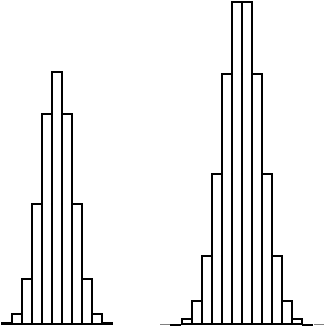
\includegraphics[scale=0.5]{FiguresMaths/ProbaGaussianDistribution}
        \caption{Distribution of the binomial coefficients in the 10th row (left) and the 15th row (right) of the Pascal's triangle.
        The scale of the right histogram is 1/20.}
        \label{fig:gaussiandistribution}
\end{center}
\end{figure}


\section{Beyond the Basics}

As students are introduced to modern topics within computing, whether
at the level of a Computing Literacy course or a post-core technical
course, they will have to master a variety of more specialized topics
that combine pieces of the elements we have discussed in this essay.
While these topics are beyond the level of generality aimed at in this
essay, some may be appropriate prerequisites to programs that have
some specialized foci.
\begin{itemize}
\item
Issues relating to {\em clustering} find application in applications as
diverse as: {\em linear-algebraic computations}, {\em data mining},
{\em design and layout of digital circuitry}.

\item
Issues building on {\em graph separation/decomposition} are
encountered when studying: {\em linear-algebraic computing}, {\em
  fault-tolerant design}, {\em load balancing}.

\item
Many issues relating to {\em fault/failure tolerance} and {\em data
  analytics} benefit from study using {\em random walks} (at least in
one dimension).

\item
Many useful ideas regarding the {\em encoding and manipulation of
  data} can be gleaned from the elements of {\em information theory}
and {\em computer arithmetic}.
\end{itemize}
The preceding list is really endless.  Hopefully readers will be
inspired by our few examples to compile a longer version that is
appropriate for their particular environments.




